\section{Metriken}

\addtocontents{toc}{\protect\setcounter{tocdepth}{1}}

Zur Auswertung der Modelle werden Metriken genutzt. Die Auswahl der richtigen Metriken hängt von der gewünschten Zielsetzung ab.
Diese kann zum Beispiel binäre, bzw. multi-Klassen Klassifikation oder Regression sein.

Fake News Erkennung ist eine binäre Klassifizierung (Der Artikel ist entweder 'wahr' oder 'falsch').

Dabei ergeben sich vier mögliche Ausgänge bei der Modellvorhersage:
\begin{itemize}
    \item True Positive (TP) - Das Modell hat die positive Klasse vorhergesagt. 
        
    (Der Artikel, der kein Fake ist, wird als 'wahr' gedeutet)
    \item True Negative (TN) - Das Modell hat die negative Klasse richtig vorhergesagt.
        
    (Der Artikel, der Fake ist, wird als 'falsch' gedeutet)
    \item Falsch positiv (FP) - Das Modell hat die positive Klasse falsch vorhergesagt. 
        
    (Der Artikel, der kein Fake ist, wird als 'falsch' gedeutet)
    \item Falsches Negativ (FN) - Dein Modell hat die negative Klasse falsch vorhergesagt. 
        
    (Der Artikel, der kein Fake ist, wird als 'wahr' gedeutet)
\end{itemize}

Diese vier Werte werden in einer sogenannten Konfusionsmatrix  (siehe Abbildung \ref{fig:confusion_matrix}) zusammengefasst
aus der verschiedene Bewertungsmetriken abgeleitet werden können.

\begin{figure}[htbp]
    \begin{center}
        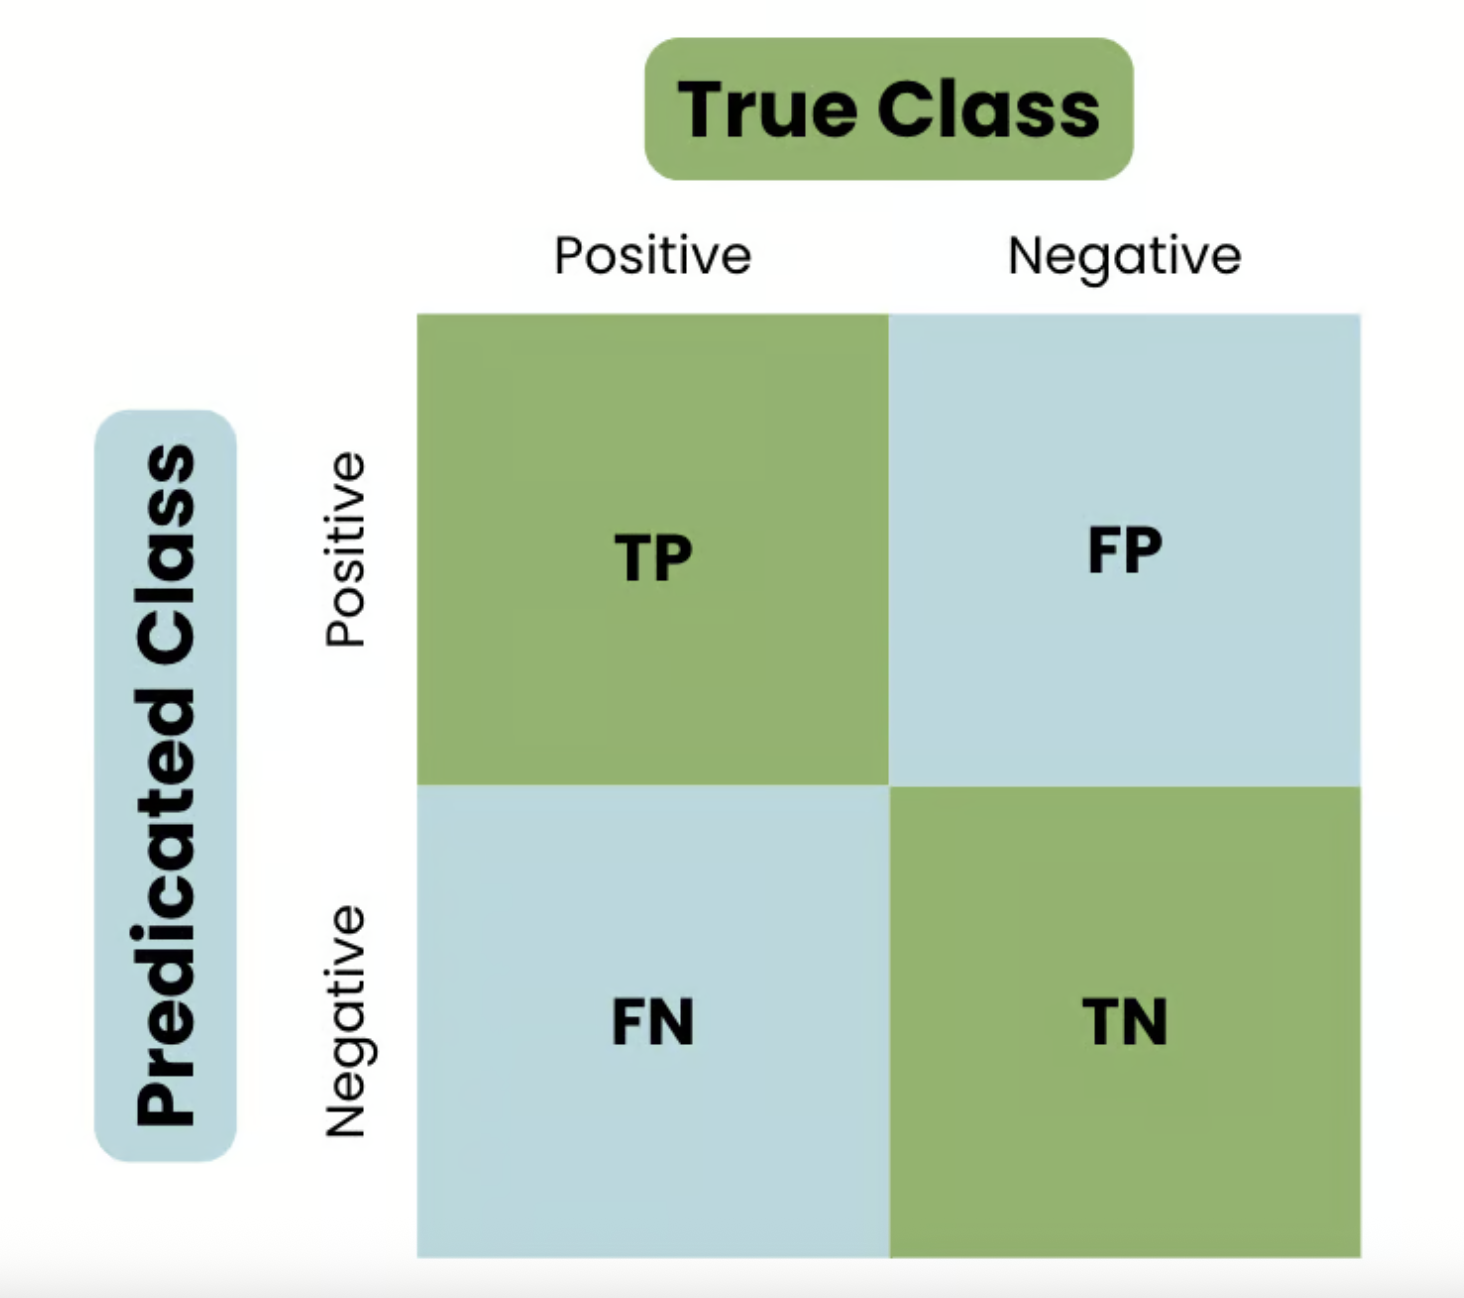
\includegraphics[scale=0.3]{static/confusion_matrix.png}
        \caption[Konfusionsmatrix]{\label{fig:confusion_matrix} Konfusionsmatrix \cite{datacamp_confusion_matrix_tutorial}}
    \end{center}
\end{figure}

Nach \cite{kivimaeki2025, Rainio:2024aa} sind die relevantesten Metriken für binäre Klassifikationen Accuracy, Recall (Sensitivity in \cite{Rainio:2024aa}), 
Specificity und Precision. 

\subsection{Accuracy}

Die Accuracy gibt den Anteil korrekt klassifizierter Instanzen an.

\begin{equation}
    \text{Accuracy} = \frac{TP + TN}{TP + TN + FP + FN}
\end{equation}

\subsection{Recall}

Der Recall gibt den Anteil korrekt erkannter positiver Fälle an.

\begin{equation}
    \text{Recall} = \frac{TP}{TP + FN}
\end{equation}

\subsection{Specificity}

Die Specificity gibt den Anteil korrekt erkannter negativer Fälle an.

\begin{equation}
    \text{Specificity} = \frac{TN}{TN + FP}
\end{equation}

\subsection{Precision}

Die Präzision gibt den Anteil tatsächlich positiver Fälle unter allen als positiv vorhergesagten Fällen an.

\begin{equation}
    \text{Precision} = \frac{TP}{TP + FP}
\end{equation}

\subsection{F1-Score}

Der F1-Score vereint die beiden Metriken Recall und Precision in einem einzigen Wert und ist hilfreich, wenn ein Gleichgewicht zwischen 
diesen beiden wichtig ist – vor allem bei unausgeglichenen Datensätzen, bei denen Accuracy allein irreführend sein kann.

Sind in dem Datensatz der Fake News Erkennung zum Beispiel 95\% der Artikel 'wahr' und 5\% 'falsch' hat ein Modell das ausschließlich
'wahr' vorhersagt eine Accuracy von 95\%. Es erkennt aber keinen einzigen Artikel der Fake ist.
Der Recall wäre in diesem Fall 0 und somit auch der F1-Score.

\begin{equation}
\text{F1\text{-}Score} = \frac{2 \cdot \text{Precision} \cdot \text{Recall}}{\text{Precision} + \text{Recall}}
\end{equation}

\addtocontents{toc}{\protect\setcounter{tocdepth}{2}}